Deep neural networks are often thought of as ``black boxes'' that are
easy to train but difficult to intepret. Interpreting the results
obtained using these techniques may indeed be more challenging than
getting the results themselves. This difficulty of interpretation
sometimes leads to the suspiction that the neural network learns
artifacts in the data that correlate with the target results but are
not meaningful by themselves.
%
In this section we attempt to show that our network learns relevant
description of a protein structure and can successfully rank decoys, 
generated by a single algorithm.
%%% GL: ``submissions between prediction groups''? I don't understand
%%% what you mean.
%G: Corrected

First, we identify the regions of a structure that are responsible for
an increase of its score (a \emph{decrease} in its quality). If the
network has learned intepretable features of the data, we expect this
analysis to show that the regions responsible for the poor quality of
a decoy structure are those in which it deviates from the native
structure.
%
We use the Grad-CAM analysis technique proposed by Selvaraju et
al.~\cite{selvaraju2016grad}. The key idea of this technique is to
compute the gradient of the model output with respect to the output of a certain layer of the network
and take the sum of the layer output weighted by the gradient.
%%% GL: ``Propagate'' is jargon, here. You mean you are calculating
%%% the gradient of the input w.r.t. the input to all nodes of a
%%% certain layer?
%G: corrected
%%% GL: ``Activation'' is also jargon. We need to explain what it is.
%
%%% GL: Why ``activations'' plural but ``gradient'' singular?
%
%%% GL: Let me try to put that in simpler words:
This highlights output regions of that layer that are both strongly
activated and highly influential on the output.
%
%%% GL: Too much jargon in the next sentence (upscaled? reception
%%% field?).
%G: corrected
The weighted layer output is then upscaled to the same size as the input of the network. 
It indicate which parts of the input contribute the most to the gradient of the network output.
%
In our case we choose the ReLU layer 10, for which
the output size is $25\times 25\times 25$.
%%% GL: This is not clear. The layer counting is not at all obvious
%%% from Figure 3 and the reader won't be able to identify which layer
%%% we're talking about.
%G: read the SI
%%% GL: Figure 3 needs to be more accurate. It should show all layers,
%%% as well as the size of each 3D grid. If I'm not mistaken, it goes
%%% 120x120x120, 118x118x118, 58x58x58, 56x56x56, 27x27x27, 25x25x25,
%%% 23x23x23, 11x11x11, 9x9x9, 7x7x7 (not shown!), 5x5x5, 3x3x3 (not
%%% shown!), 1x1x1.
%G: The precise table is shown in the SI. It's too big for the manuscript itself
We tested the method on the outputs of the neighboring layers and
layer 10 represents the best tradeoff between interpretability and
coarseness.
%%% GL: Best? Did you try other layers?
%G: yes
An example of the output is given in Fig.~\ref{Fig:GradCAMT0776}
%%% GL: Are the results for this particular target typical?
%G: yes
In line with our scoring procedure, we perform the Grad-CAM analysis
by uniformly sampling 100 rotations and translations of the decoys. We
obtain the weighted layer outputs for each of the transformations sampled and
project them onto the atoms of the
decoy. Figure~\ref{Fig:GradCAMT0776} shows two representations of such
an average weighted layer outputs (for decoy Distill\_TS3 of target T0776): a
projection of the map onto the atoms of the decoy, represented as a
color-coded value on the cartoon rendering of the structure, and a
projection onto a 3D grid, represented as an isosurface. The
isosurface of Fig.~\ref{Fig:GradCAMT0776} is a hollow shell containing
most of the solvent exposed region of the decoy, which indicates that
the network enforces packing: any increase in the atomic density
around the well-packed core decreases the quality of the decoy.
%
Strikingly, we find that the weighted layer outputs are mostly zero for
structures close to the native ones (results not shown), despite the
fact that no gradient information was included in the training
procedure. 
%This suggests that the model has learned a score $f$ that
%plays a role similar to a free energy of folding and becomes minimum
%for the native structure.
%G: not justified

Figure~\ref{Fig:GradCAMT0776_more} shows the color-coded
values of the weighted outputs for four decoys of target T0776.
%%% GL: Discussion of these results???
%G: 
%>The
%>isosurface of Fig.~\ref{Fig:GradCAMT0776} is a hollow shell containing
%>most of the solvent exposed region of the decoy, which indicates that
%>the network enforces packing: any increase in the atomic density
%>around the well-packed core is penalized.


\begin{figure}[H]
    \centering
    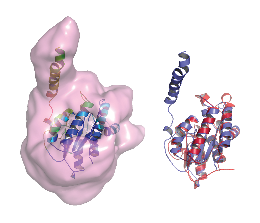
\includegraphics[width=0.5\linewidth]{Fig/FigT0776.eps}
%
    \caption{Left: Upscaled gradient-weighted outputs of the layer 10 of the network for
    candidate structure Distill\_TS3 of target T0776. The isosurface
    shows the scaled outputs at the two-sigma level. The intensities
    of the outputs at the positions of the protein atoms are
    color-coded on the cartoon rendering of the structure, from blue
    (low intensity) to red (high intensity). Right: Cartoon
    representation of the Distill\_TS3 decoy structure (in blue)
    aligned to the native structure (in red).}
%%% GL: Why do you say ``*scaled* gradient-weighted activation map''?
%%% The figure would look exactly the same if the maps were not
%%% scaled.
%
    \label{Fig:GradCAMT0776}
\end{figure}

\begin{figure}[H]
    \centering
    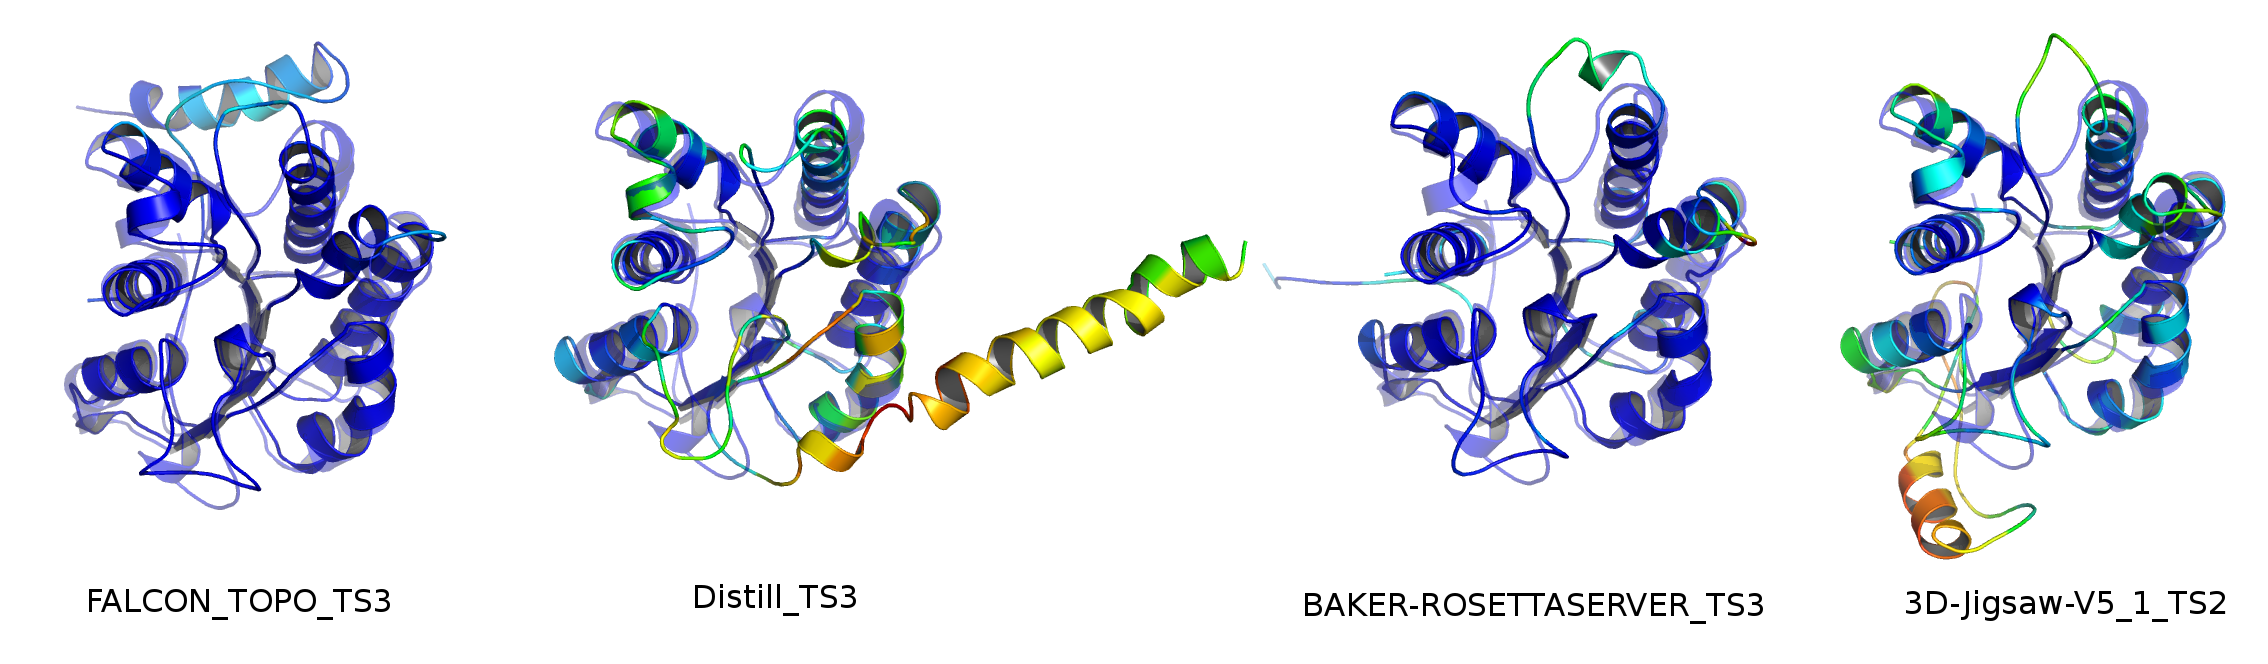
\includegraphics[width=\linewidth]{Fig/T0776.eps}
%
    \caption{Upscaled gradient-weighted outputs of the layer 10 of the network
    projected onto the atoms of the decoys. Each decoy is aligned to
    the native structure, shown as a transparent, blue cartoon.}
%%% GL: Why ``scaled''?
%
    \label{Fig:GradCAMT0776_more}
\end{figure}

To verify that the network we trained does not rely on artifacts in
the data to rank decoys, we have assessed its performance on a second,
independent dataset generated by the 3DRobot
algorithm \cite{deng20163drobot}. The decoys generated by this
algorithm are uniformly distributed within RMSD range of $[0; 12\AA]$
of the native structure and are optimized for the number of hydrogen
bonds and compactness.
%%% GL: What do you mean? They maximize the number of HBs and the
%%% compactness?
%
The dataset consists of 300 decoys for each of the 200 non-redundant proteins. The proteins were 
selected from the PDB database with less than 20\% pair sequence identity, containing 48 $\alpha$, 
40 $\beta$ and 112 $\alpha/\beta$ signle-domain proteins with length from 80 to 250 residues. 
%%% GL: Why targets are you using? How many decoys per target? You
%%% need to explain better what that second dataset is.
%G: added
The absolute \tchanged{Pearson} $R$ coefficient averaged per-target over all the
targets in this benchmark was $0.85$. Spearman $\rho$ coefficient
and Kendall $\tau$ coefficient were $0.83$ and $0.64$, respectively.
Representative examples of scoring funnels are shown in
Fig.~\ref{Fig:3DRobotBenchmark}.  We see, that the MQA method devised
in this work successfully ranks unrelated datasets.
%%% GL: What do you mean? What hyperparameters? What generator?
%G: removed it

\begin{figure}[H]
    \centering
    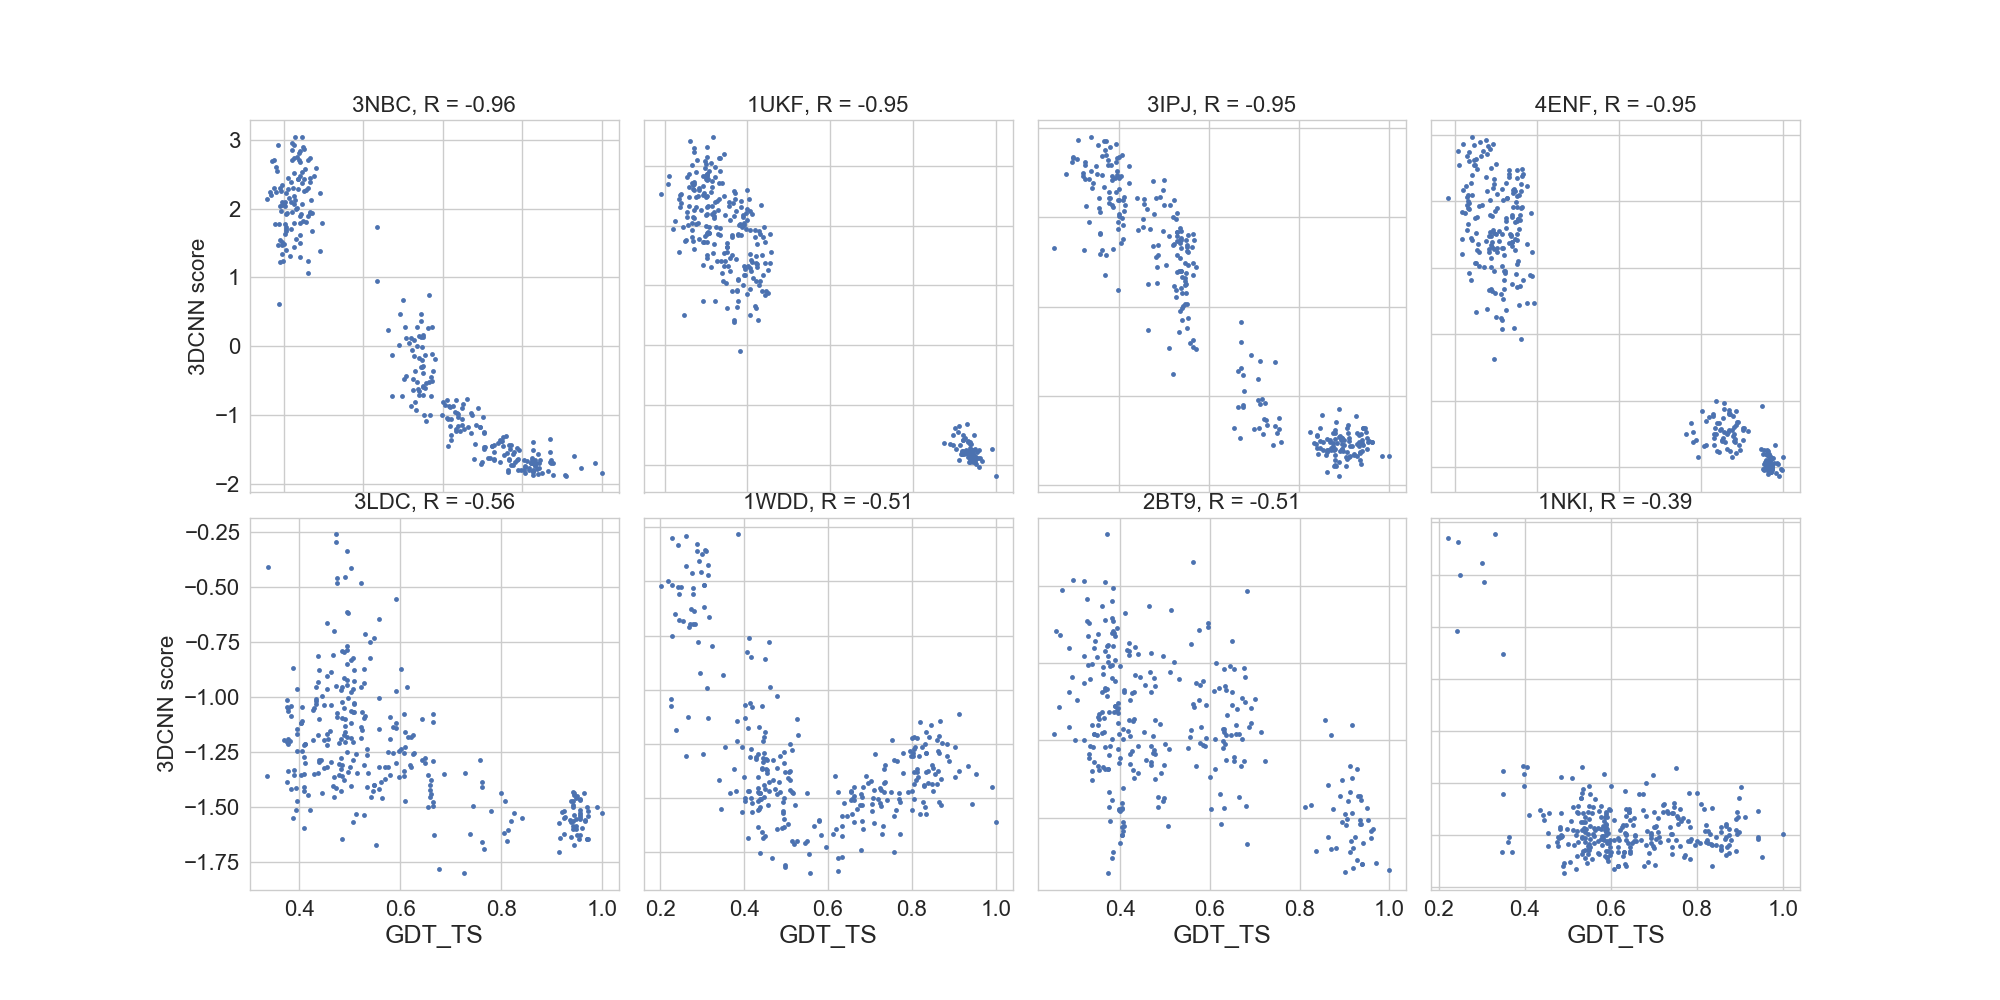
\includegraphics[width=\linewidth]{Fig/3DRobot_set_sFinal_funnels.eps}
%
    \caption{The plots of score versus GDT\_TS for four best correlated targets and four
    least correlated targets in the 3DRobot benchmark.}
%%% GL: You don't explain what a ``scoring funnel'' is.
%G: corrected
    \label{Fig:3DRobotBenchmark}
\end{figure}
